\chapter{Dependency Injection}

%% Essa primeira parte está bem ruim, Tenho q revisar, mas é preciso começar em algum lugar...

Since the inception of object-oriented programming the start-up of applications has always been troublesome.
This is because the greatest contribution of object orientation, which is polymorphism, is difficult to
apply effectively for object instantiation and configuration. Basically, polymorphism is the process of 
abstracting away the implementation of an object behind a well-known interface, so different
implementations of an interface with different behaviors can be treated uniformly. As a consequence a client
object can use another object only knowing its interface. The problem is how does it obtain a reference to
the other object? There are only two options: either the object itself tries to obtain it or the reference is configured externally. 

Let us analyze the first option. The easiest option is to instantiate directly using the appropriate language primitive.
The problem with this approach is that to instantiate an object it is necessary to know its concrete implementation type.
This works in many cases but all the benefits of polymorphism are negated because the client object is no longer
independent of the implementation of the other object. 

Another option is to delegate the instantiation or look-up to another object. In this case first a reference to the factory object
must be obtained and then it can be used to build or look-up the other object. Now the client object is no longer dependent on the
concrete type of the other object. But we are back to the exact same problem: how do we obtain a reference to the factory object?
It's clear that we cannot go on and on creating factories of factories. Usually this cycle is broken by employing the singleton pattern
to make the factory object unique and globally accessible. The benefit of this practice is that the factory object can be configured
to create different implementations depending on the applications needs. The problem of this approach is that the object now depends
on two interfaces: the interface of the object it needs to do its work and the interface of the object needed to provide the reference
of the other object. And no matter how hard we work to abstract away the instantiation, the unwanted coupling to a third party will always
be there. And matters get worse when we think of modularity. How can an object that depends on a factory be distributed for reuse?
The factory must be distributed as well.

All the problems of the first approach approach boil down to this: making an object responsible for its own composition. Seen this way it doesn't make
sense at all. An electronic component does not search for the other components on the circuit board it should interact with: it just assumes
they are there. And this leads to the second approach: external composition. Following this approach objects are programmed to declare the dependencies
on external interfaces. Then, at application start-up, all objects are instantiated and wired one to another. This approach is often called dependency
injection or inversion of control.

\section{The benefits of dependency injection}

\subsection{Reuse}

In the discussion above one problem of the factory or service locator pattern was that objects in one way or another were tied to a factory
implementation. This means that they cannot be used independently of the factory object. In contrast, using dependency injection the object
depends solely on the abstract interface of other objects it collaborates with and can be reused independently.

\subsection{Modularity}

The fact that objects are tied to a factory impacts its physical packaging as well. We can put the factory in the unit of
deployment or in a separate one. In the second case we end up forcing a dependency between physical modules as well.
Using dependency injection, a module can contain only the classes that implement the desired functionality without being
tied to other modules.

In some cases it is possible to deliver a component and it the factory of its dependencies in the same physical modules
but in other cases it is desirable to reuse the service object and its factory in several different context justifying its
location in a separate module. Now consider what happens if we have to make changes to the factory's interface. All other
modules that depend on this module will have to be changed as well.

\subsection{Intentionality}

Intentionality is a subjective code measure that captures to what degree it is possible to understand the specification
of a piece of code only by reading it. It is defined by Armstrong as follows:

\begin{quotation}
Intentional Programming - this is a programming style where the programmer can easily see from the code exactly
what the programmer intended, rather than by guessing at the meaning from a superficial analysis of code
\end{quotation}


Another definition is given by Czarnecki:

\begin{quotation}
... decrease the conceptual gap between program code and domain concepts (known as achieving high intentionality)...
\end{quotation}

We say that intentionality is subjective because it is influenced by a several factors such as the familiarity of
the reader with the programming language and libraries being used and the overall structure of the code. Despite
this subjectivity it should be clear that if a piece of code is cluttered with secondary concerns it will be
less understandable and therefore have a lower intentionality. This has to do with the principle of separation of
concerns as is explained very lucidly by Czarnecki:

\begin{quotation}
One of the most important principles of engineering is the principle of separation of concerns.
The principle acknowledges that we cannot deal with many issues at one, but rather with one at a
time. It also states that important issues should be represented in programs intentionally (explicitly, declaratively)
and well localized. This facilitates understandability, adaptability, reusability, and the many other good qualities 
of a program since intentionality and localization allow us to easily verify how a program implements our requirements.
\end{quotation}

We believe that dependency injection increases the intentionality of code because the concern of locating external components
is separated from the task that a piece of code is written to accomplish. Also the dependency on external components is explicitly
represented in the external representation of a concrete class. For example in Java references are represented as attributes or
pairs of accessor methods and are subject to introspection.

Also, as will be discussed more thoroughly in the chapter about \texttt{SCA}, dependency injection has the potential to remove
direct code dependencies on the component framework being used and which further helps to simplify the code.

\subsection{Portability}

In many situations programming frameworks act as factories or service locators. For example components built on top of CCM
explicitly call the CCM framework to locate other components. This means that CCM components are tightly coupled to
the CCM runtime and cannot be reused in other situations. In other words, they are not portable. In contrast, if we look at
applications developed using the Spring Framework for Java we will see that they are POJOs that never reference Spring's API
and can therefore be used in other contexts.

\begin{center}
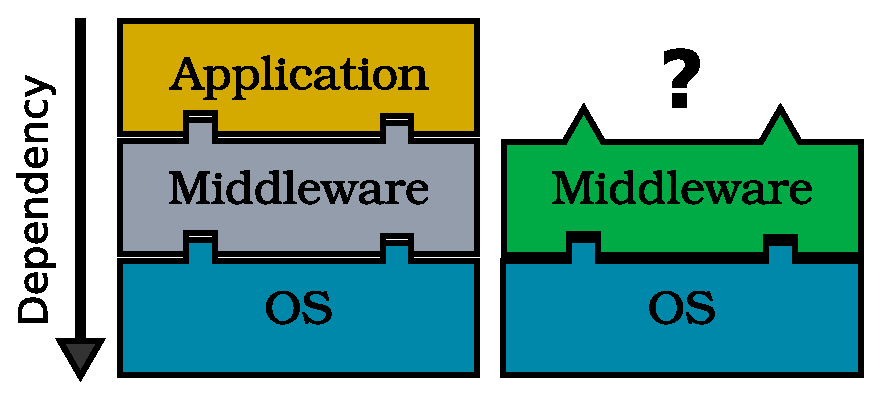
\includegraphics[height=80pt]{graphics_tables/bad_layers.eps} 
\end{center}

The problem with the earlier component framework is that they are based on a strictly layered approach. Traditionally systems
are structured in layers where the more abstract layers depend on more the concrete layers below them. The benefit is that
the higher level layers can be built without worrying about low-level concerns. The drawback is that the higher level
layers are tightly coupled to the layers directly below them and are usually not portable to other stacks.
This problem can be mitigated by creating standards for the API of a layer, like \texttt{POSIX}, but cannot be completely
eliminated. 

With inversion of control, the infra-structure can sometimes be abstracted away completely eliminating source dependencies
on infra-structure APIs. As will be explained in the chapter about \texttt{SCA}, dependency injection can be used to adapt
a generic component to a specific middleware platform.

\begin{center}
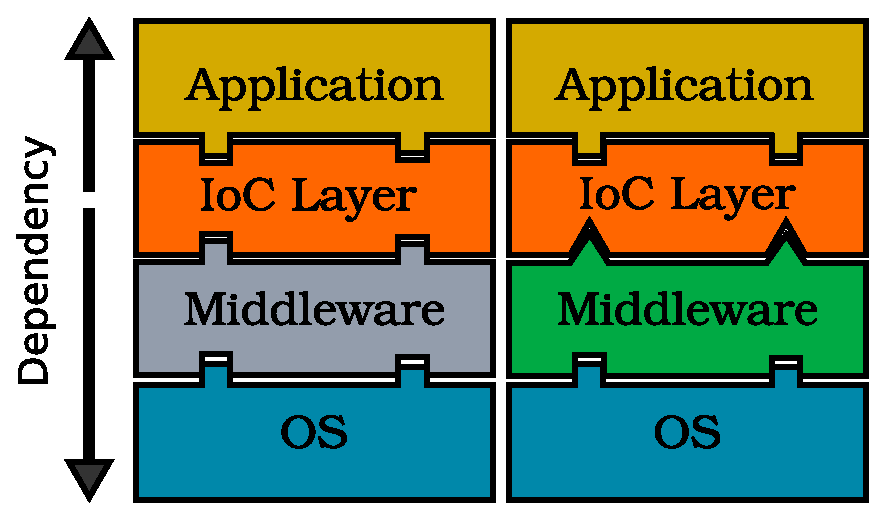
\includegraphics[height=80pt]{graphics_tables/good_layers.eps} 
\end{center}


\subsection{Interoperability}

Component frameworks like CCM are created to foster the reuse of software components. Unfortunately these component frameworks are
incompatible: a component in a CCM container cannot use a COM component directly. So the platforms created to enable reuse can actually
hinder it in some situations, creating islands of compatibility. 

There are several solutions to bridge the gap between different middleware platforms such as the translation of network protocols.
But it would be even better if the component framework to use was just a matter of external configuration. Then we could take two
components and configure the remote method invocation protocol they should use to talk to each other.

\section{Requirements of dependency injection and implementations}

Dependency injection, as a principle, can be applied in any object oriented programming language. All it takes is to have
a piece of code that acts as a start-up script where the compositions and configurations are defined. But it is often better
to have a domain specific language for this task.

